% 2nd Milestone
\documentclass[12pt]{article}

\usepackage[a4paper,margin=0.85in,footskip=0.25in]{geometry}
\usepackage{tikz}
\usepackage{amsmath}
\usepackage{palatino}
\usepackage{setspace}
\usepackage{pgfplots}
\usepackage{graphics}
\usepackage{dirtytalk}
\usepackage{dramatist}


\pgfplotsset{compat=1.16}
\bibliographystyle{plain} % Change this to your desired style
% \addbibresource{sources.bib}


\begin{document}
\noindent
Aidan LaBella \\
DATA/EEPS 1720 \\
Project Milestone 3\\
4/18/2024 \\

\textbf{Forecasting Air Quality Metrics With Evolved Recurrent Neural Networks}

\section{Introduction}
The main question my project attempts to answer is \say{can we \textbf{forecast} air quality data when sensor data is unreliable and/or not present}? This project, at a high level, is to train a model that is effective at predicting air pollution given certain parameters. I also propose using a toolkit for neural architecture search while training the model. The applications of a model that can predict air quality vary from being able to estimate the pollutants in the air based on other parameters, to being able to accurately forecast when the pollution will reach its high/low levels, much like a weather forecast. 

Recurrent Neural Networks, or RNNs are an effective way to regress over a dataset. Since RNNs are able to output a set of parameters for a variable number of time-steps, this makes them ideally suited for time series forecasting as opposed to time series classification \cite{yang2022predictive}. Air quality data takes the form of hourly readings from sensors that measure different contents of elements in the air. As such, RNNs can be said to be well-suited for this type of time series forecasting. However, one of the drawbacks that RNNs bring is a computational overhead due to their need to be “unrolled” through time. Because of this, creating smaller recurrent neural networks has been a priority in the DL field but finding the right architecture has been a challenge. Using the Evolutionary eXploration of Augmenting Memory Models (EXAMM)\cite{ororbia_investigating_2019}, we can “evolve'' recurrent neural networks to (hopefully) be the “smallest” yet best performing model for a given task. Not only does this reduce the complexity of the model, it can reduce the computational cost which in turn makes the model more environmentally friendly. We will show that our evolved networks can achieve the same levels of performance as a traditional RNN in PyTorch or Tensorflow.

\section{Related Work}
Previous applications of the EXAMM\cite{ororbia_investigating_2019} toolkit with neural architecture search (NAS) include making predictions for coal power plants\cite{kaufmann_evolving_2019}. We seek to use this work as a foundation and proof-of-concept for our task of forecasting air quality data. 
\subsection{The EXAMM toolkit}
The EXAMM toolkit was developed by the Distributed Data Science Systems lab (D2S2) at Rochester Institute of Technology, before the \say{explosion} of modern neural network frameworks like PyTorch and Tensorflow. EXAMM is written entirely in C++ and utilizes cpu-bound MPI and multithreaded compute methods in lieu of GPUs. EXAMM also focuses on feed-forward and recurrent neural networks for its evolutionary processes. This is due to the fact that neuro-evolution for CNNs is a bit trickier to conduct due to the intensive computational resources required for training and evaluation. One added benefit of a NAS apparoach is its ability to identify the necessary input columns for a successful prediction. In turn, this will allow us to answer \textbf{RQ1}.

\begin{figure}
    \begin{center}
        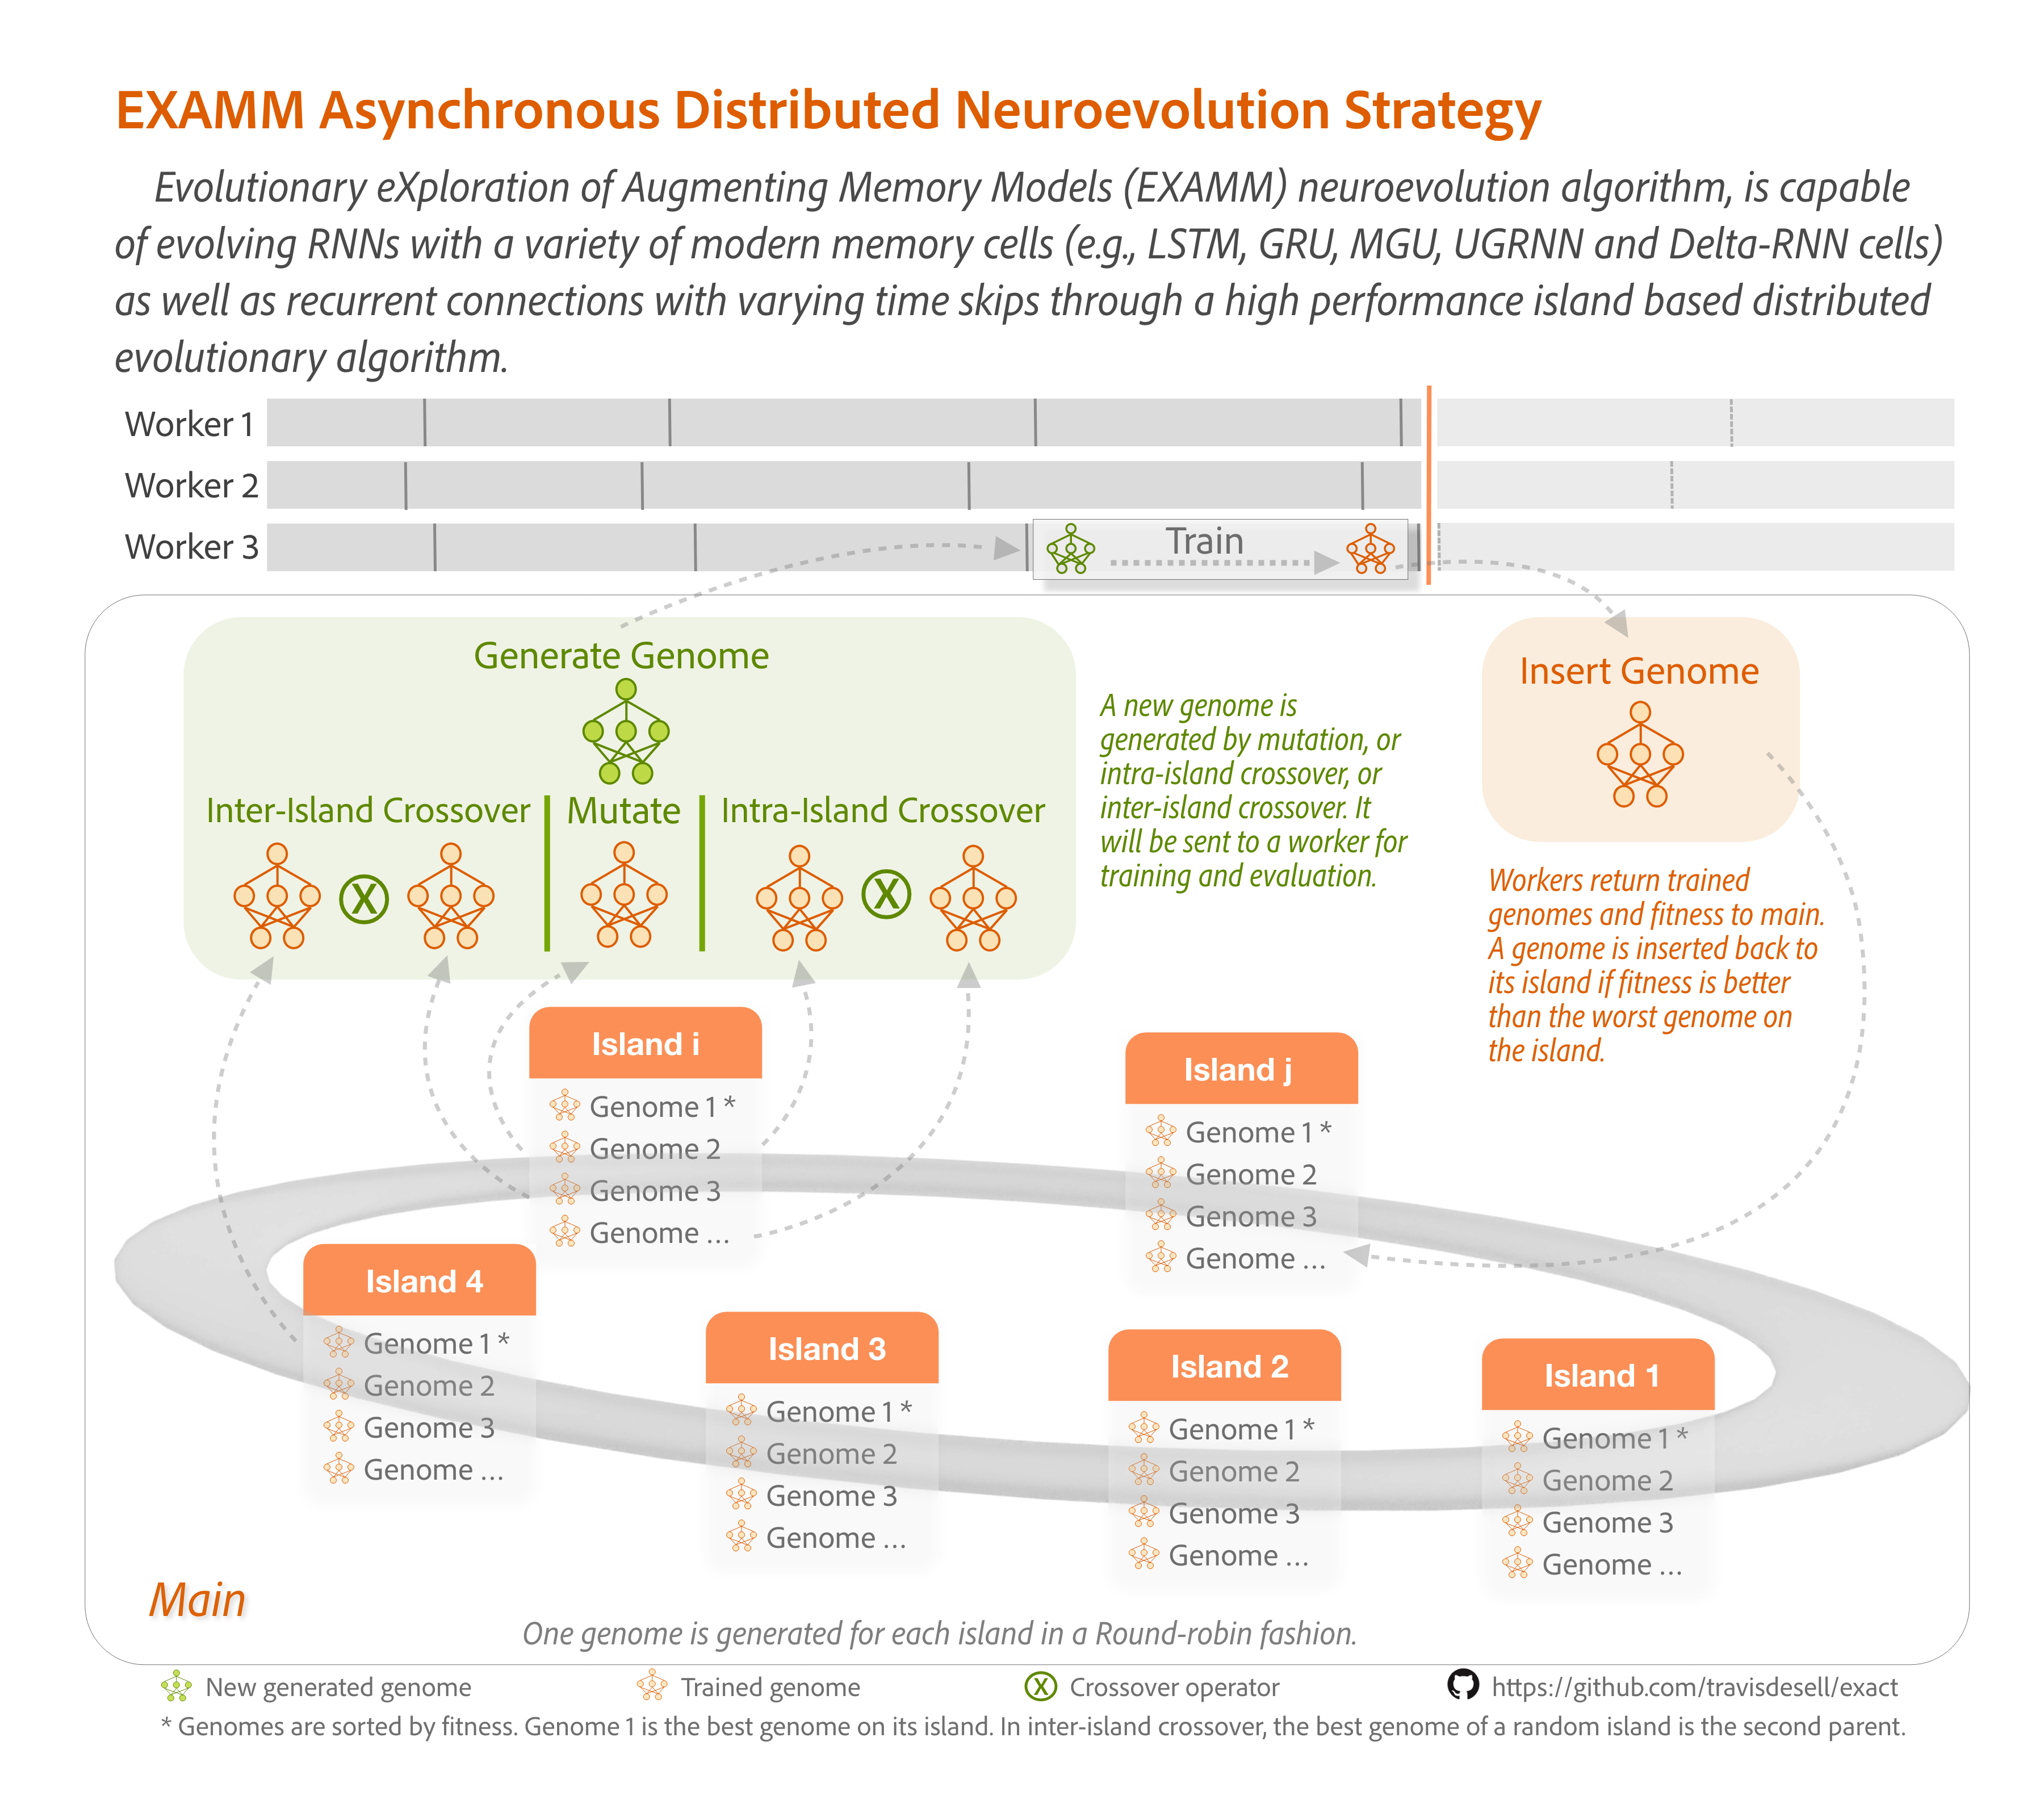
\includegraphics[width=0.95\textwidth]{resources/EXAMM.png}
    \end{center}
    \caption{EXAMM's evolutionary process \cite{lyu2023online}}\label{fig:examm}
\end{figure}


\section{Dataset(s)}
For this project, multiple datasets were explored including the UCI Air Quality repository and the NASA MERRA-2 dataset.
\subsection{UCI Air Quality}
It is important to first note that this work can be classified as a multivariate time series classification forecasting task. The data that will be used to train the models will be multivariate in form, with one or more columns potentially missing or corrupted to simulate unreliable data.
To train a well-performing recurrent neural network, we must first find a well-curated dataset that has enough sensor readings to learn from. The UC Irvine Air Quality dataset \cite{misc_air_quality_360} uses 9358 instances of hourly averaged responses from an array of 5 sensors within an Italian city from March 2004 to February 2005, approximately 1 year in time.
\subsection{MERRA-2} 
The MERRA-2 \cite{gelaro2017modern} dataset was chosen as a more complete and representative dataset with regard to US air quality. For the purposes of this project, we will look at the following columns:
    \begin{table}[h]
    \centering
    \begin{tabular}{|c|p{10cm}|}
        \hline
        \textbf{Parameter} & \textbf{Description} \\
        \hline
        \hline
        AIRDENS & Air density, in kilograms per cubic meter (kg/m\textsuperscript{3}) \\
        \hline
        SO4 & Sulfate concentration in micrograms per cubic meter ($\mu$g/m\textsuperscript{3}) \\
        \hline
        SO2 & Sulfur dioxide measured in parts per billion (ppb) \\
        \hline
        RH & Relative humidity as a percentage \\
        \hline
        PS & Atmospheric pressure, in hectopascals (hPa) or millibars (mbar) \\
        \hline
        H & Hydrogen concentration, in parts per million (ppm) \\
        \hline
        O3 & Ozone concentration, in parts per billion (ppb) \\
        \hline
        T & Temperature of the air, in Kelvin (K) \\
        \hline
        U & Horizontal wind speed, meters per second (m/s) \\
        \hline
        V & Vertical wind speed, in meters per second (m/s) \\
        \hline
        CO & Carbon monoxide concentration in parts per million (ppm) \\
        \hline
    \end{tabular}
    \caption{Glossary of MERRA-2 Parameters}
    \label{tab:merra-params}
\end{table}
\paragraph{Parameter Forecasting} To have a meaningful measure of the air quality at a given point in time, we will narrow our focus to the following particulate air measures. Our main focus will be on CO levels but for mutivatiate output layers we will look at additional parameter levels. We will focus on Carbon Monoxide (CO) for our univariate predictions as it's harmful effects are well-known and researched \cite{rose2017carbon}.
\begin{enumerate}
    \item
        CO or Carbon Monoxide
    \item
        O3 or Ozone Concentration
    \item
        SO$_{4}$ or Sulfate Concentration
    \item
        SO$_{2}$ or Sulfur Dioxide Concentration
\end{enumerate}

\section{Exploratory Analysis}
For a \say{proof of concept}, the entire dataset was used to \say{evolve} network(s) and evaluate their performance. In NAS, evolution refers to the process of augmenting the model's architecture through random mutations, followed by gradient descent for adequate evaluation. In the experiments conducted, we attempt to impute the ground truth readings based on date, time, temperature and other sensor readings. We evolve the networks for 2000 genomes (series of mutations) with 5 epochs of gradient descent for evaluation. The preliminary MSE values of well-performing genomes (models) for univariate ouputs has been found to be in the ballpark of $[.02,.04]$, an acceptable range for any deep learning model. For multivariate outputs, the loss was higher ($\geq 0.2$). Thus, I am confident that an evolved RNN will be well-suited to make predictions for this task. 

\section{Methodology}
The methodology of this work will focus around the following research questions:
\paragraph{RQ1:} What input columns can accurately estimate the levels of pollutants such as Carbon Monoxide, $CO$? \\
\paragraph{RQ2:} Can multiple prediction columns exist in the output layer with minimal performance impact? I.e. can we predict multiple columns at once? \\
\paragraph{RQ3:} How do our \textbf{forecasted} values compare with actual sensor readings?\\
\paragraph{RQ4:} What is the inference time of the best performing model? How does it compare to a standard Jordan, Elman and standard RNNs? \\
Since one of the goals of this project is to be able to forecast air quality parameters
\subsection{Multivatiate Output Layer}
% For predicting multiple air quality data points, such as CO, SO_{4}, SO_{2} and O_{3}, we will use the following input parameters:\\
\subsection{Univariate Output Layer}


\section{Evaluation}
To evaluate both \textbf{RQ1} and \textbf{RQ2}, both mean average error (MAE) and mean squared error (MSE) will be used. 
This aims to answer \textbf{RQ1} \& \textbf{RQ3}.

\section{Acknowledgments}
I want to thank my B.S. advisor, Dr. Travis Desell and my former lab-mates, Josh Karns and Zimeng Lyu at RIT for their help and support with the EXAMM code base!

\bibliography{sources} % Replace with your BibTeX filename
\end{document}
